\section{Semaine 6 : 13/03/2023 - 17/03/2023}
\graphicspath{{semaines/semaine_6/images/}}


\begin{abstract}
	Après les tests de la semaine dernière sur la partie de correction/certification du modèle où l'on prend la solution analytique comme nouvelle level-set, il semblerait que la méthode avec les meilleurs résultats soit celle où l'on utilise la méthode extrapolate de FEniCS. C'est pourquoi, cette semaine on s'est intéressé en détail au code source de cette fonction FEniCS (\href{https://fenics.readthedocs.io/projects/dolfin/en/2017.2.0/apis/api_adaptivity.html#extrapolation}{Extrapolation}). Étant donné que je n'étais pas présente mardi, mercredi après-midi et jeudi car j'étais malade, c'est tout ce qui a été fait cette semaine. De plus, une grosse partie de la méthode reste encore floue : la construction de la matrice A (pour la résolution du système linéaire dans compute\_coefficients).
\end{abstract}

Pour illustrer les explications, nous considérerons un domaine rectangulaire maillés uniformément par des triangles. Dans la suite, nous considérerons également \textit{cell0} comme étant une des cellules de maillage. On prendra comme exemple une extrapolation de $\mathbb{P}^1$ vers $\mathbb{P}^2$. 

\begin{minipage}{0.48\linewidth}
	\begin{figure}[H]
		\centering
		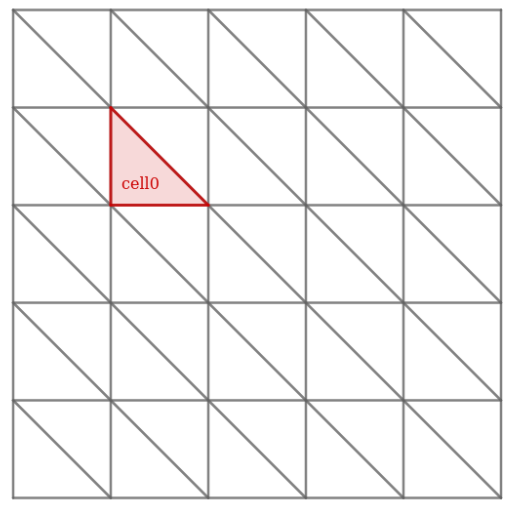
\includegraphics[width=0.5\linewidth]{cell0.png}
		\caption{Cell0}
	\end{figure}
\end{minipage}
\begin{minipage}{0.48\linewidth}
	\begin{figure}[H]
		\centering
		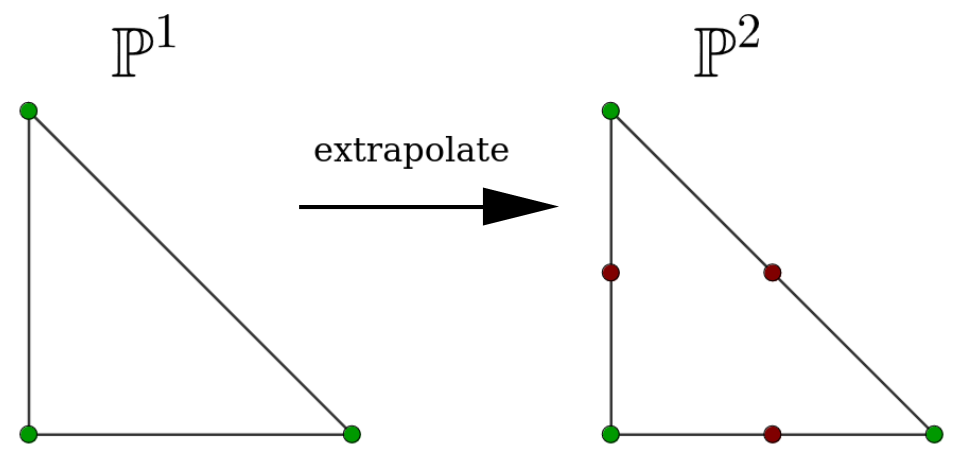
\includegraphics[width=0.9\linewidth]{P1toP2.png}
		\caption{Extrapolation de $\mathbb{P}^1$ vers $\mathbb{P}^2$}
	\end{figure}
\end{minipage} \; \\


Corps de la fonction \textbf{extrapolate} qui a pour but d'extrapoler la fonction $v$ en une fonction $w$:

\begin{lstlisting}
	void Extrapolation::extrapolate(Function& w, const Function& v)
\end{lstlisting}

On cherche à calculer la valeur en chacun des degrés de liberté associé à la fonction $w$. Pour cela, on va parcourir toutes les cellules du maillage dans le but de construire le tableau \textit{coefficients} (de taille le nombre total de degrés de liberté associés à $w$). On appelle alors sur chacune des cellules la fonction \textbf{compute\_coefficients}~\ref{compute_coefficients} qui va compléter le tableau \textit{coefficients} aux indices associées à ses degrés de liberté. Comme les degrés de liberté d'une cellule peuvent être communs à ceux d'une autre, on finira par faire une moyenne des coefficients en chacun des degrés de liberté en utilisant la fonction \textbf{average\_coefficients}~\ref{average_coefficients}, ce qui nous donne alors la fonction $w$. 

On notera que deux espaces de fonctions sont créés dans la fonction extrapolate : l'espace V est notre espace de départ (dans l'exemple l'espace $\mathbb{P}^1$) et W est l'espace d'arrivée (espace $\mathbb{P}^2$). On prendra $v\in V$ et $w\in W$.

\subsection{compute\_coefficients}
\label{compute_coefficients}

Corps de la fonction :

\begin{lstlisting}
	void Extrapolation::compute_coefficients(
	std::vector<std::vector<double>>& coefficients,
	const Function& v,
	const FunctionSpace& V,
	const FunctionSpace& W,
	const Cell& cell0,
	const std::vector<double>& coordinate_dofs0,
	const ufc::cell& c0,
	const Eigen::Ref<const Eigen::Matrix<dolfin::la_index, Eigen::Dynamic, 1>> dofs,
	std::size_t& offset)
\end{lstlisting}

Cette fonction a pour but de compléter le tableau \textit{coefficients} aux indices associées aux degrés de liberté d'une cellule donnée \textit{cell0}. Autrement dit, on cherche à déterminer les valeurs aux degrés de liberté de la cellule \textit{cell0} en utilisant l'information que nous apporte les cellule voisines à celle-ci.\\

On commence par construire les tableaux \textit{cell2dof2row} et \textit{unique\_dofs} en utilisant la fonction \textbf{build\_unique\_dofs}~\ref{build_unique_dofs}. L'ensemble \textit{unique\_dofs} contient tous les degrés de liberté de notre espace de départ $V$ (associé à la fonction $v$) des cellules voisines à \textit{cell0}. Le dictionnaire \textit{cell2dof2row} permet d'associer à chaque degré de liberté (unique) d'une cellule donnée un numéro de ligne unique. 

Ensuite, on définit $N$ le nombre de degré de liberté associé à un élément de $W$ (dans notre cas $N=6$) et $M$ le nombre de degré de liberté (unique) des cellules voisines à la cellule courante \textit{cell0} (dans notre cas les nœuds des cellules voisines et donc $M=12$). Attention : il faut que $M\ge N$ pour avoir suffisamment de degré de libertés pour pouvoir construire l'extrapolation.

On peut maintenant créer la matrice $A$ (de taille $M\times N$) et le vecteur $b$ (de taille $M$). En parcourant les cellules voisines de la cellule courante \textit{cell0}, on va compléter la matrice $A$ et le vecteur $b$ en utilisant la fonction \textbf{add\_cell\_equations}~\ref{add_cell_equations}. A noter que la cellule courante \textit{cell0} est inclue dans ses cellules voisines.

On pourra ensuite résoudre le système linéaire $Ax=b$ qui nous donnera la valeur en chacun des degrés de liberté de la cellule courante \textit{cell0}. Ces valeurs sont alors ajoutées au tableau global \textit{coefficients} qui nous fournit après avoir utilisé la fonction \textbf{average\_coefficients}~\ref{average_coefficients} les valeurs en chaque degré de liberté de $w$.

\subsection{build\_unique\_dofs}
\label{build_unique_dofs}

Corps de la fonction :

\begin{lstlisting}
	void Extrapolation::build_unique_dofs(
	std::set<std::size_t>& unique_dofs,
	std::map<std::size_t, std::map<std::size_t, std::size_t>>& cell2dof2row,
	const Cell& cell0,
	const FunctionSpace& V)
\end{lstlisting}

Cette fonction a pour but de compléter les tableaux \textit{cell2dof2row} et \textit{unique\_dofs} donnés en entrée. A noter que au total, on a le même nombre de degré de liberté dans \textit{cell2dof2row} et \textit{unique\_dofs}.\\

On commence par remplir un ensemble contenant les cellules voisines à \textit{cell0}. Pour être plus précis, les cellules voisines à \textit{cell0} sont les cellules ayant un nœud commun avec la cellule courante \textit{cell0} (Figure~\ref{fig3}).

En parcourant ensuite chacune de ces cellules, on va pouvoir compléter les tableaux \textit{cell2dof2row} et \textit{unique\_dofs} donnés en entrée en appelant la fonction \textbf{compute\_unique\_dofs}~\ref{compute_unique_dofs}. 

Dans le cas de notre exemple, on va numéroter tous les nœuds des cellules voisines à \textit{cell0} et on supposera que le parcours des cellules est effectuées dans un ordre précis (Figure~\ref{fig4}).

Alors le set \textit{unique\_dofs} contiendra tous les noeuds des cellules voisines à \textit{cell0} : 
$$unique\_dofs = \{n1,n2,n3,\dots,n12\}$$

Et le dictionnaire \textit{cell2dof2row} associé à \textit{cell0} est construit de la manière suivante :
$$cell2dof2row = \begin{aligned}[t]
	\{\quad&"cell0":\{"n1":0,"n2":1,"n3":2\},&& \\
	&"cell1":\{"n4":3\}, \\
	&"cell2":\{"n5":4\}, \\
	&\dots &&\}
\end{aligned}$$

\begin{minipage}{0.48\linewidth}
	\begin{figure}[H]
		\centering
		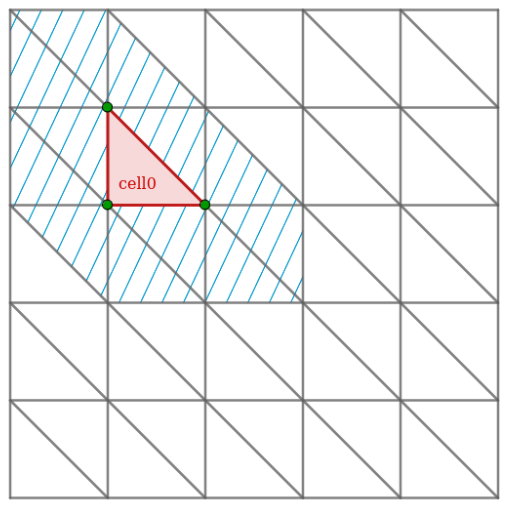
\includegraphics[width=0.6\linewidth]{surrounding_cells.png}
		\caption{Cellules voisines à Cell0}
		\label{fig3}
	\end{figure}
\end{minipage}
\begin{minipage}{0.48\linewidth}
	\begin{figure}[H]
		\centering
		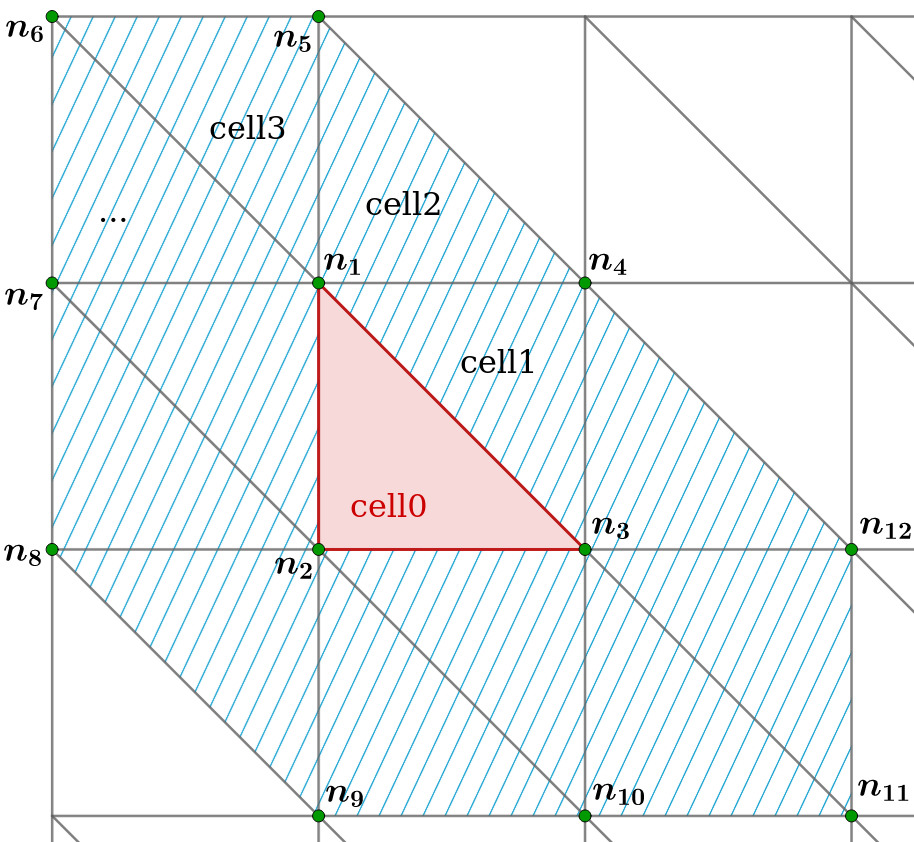
\includegraphics[width=0.6\linewidth]{cell2dof2row.png}
		\caption{Parcours des cellules voisines}
		\label{fig4}
	\end{figure}
\end{minipage}


\subsection{compute\_unique\_dofs}
\label{compute_unique_dofs}

Corps de la fonction :

\begin{lstlisting}
	std::map<std::size_t, std::size_t> Extrapolation::compute_unique_dofs(
	const Cell& cell,
	const FunctionSpace& V,
	std::size_t& row,
	std::set<std::size_t>& unique_dofs)
\end{lstlisting}

Cette fonction a pour but de traiter chacune des cellules voisines afin de compléter les tableaux \textit{unique\_dofs} et \textit{cell2dof2row} créés dans \textbf{compute\_coefficients}~\ref{compute_coefficients}.\\

Pour une cellule \textit{cell} (voisine à \textit{cell0}), on va parcourir chacun de ses degrés de liberté associé à l'espace $V$. Autrement dit, on parcourt tous les degrés de liberté dont la valeur est connue (dans notre cas les degrés de liberté $\mathbb{P}^1$ et donc les noeuds de la cellule). Si ce degré de liberté fait partie de \textit{unique\_dofs}, on ne fait rien. Sinon, on l'ajoute à \textit{unique\_dofs}. On va également créer un tableau \textit{dof2row} qui a pour but d'associer un degré de liberté à un numéro de ligne unique. Ce dictionnaire \textit{dof2row} est retourné par la fonction et permet de remplir le dictionnaire plus général \textit{cell2dof2row} créé dans \textbf{compute\_coefficients}~\ref{compute_coefficients}.

\subsection{add\_cell\_equations}
\label{add_cell_equations}

Corps de la fonction :

\begin{lstlisting}
	void Extrapolation::add_cell_equations(
	Eigen::MatrixXd& A,
	Eigen::VectorXd& b,
	const Cell& cell0,
	const Cell& cell1,
	const std::vector<double>& coordinate_dofs0,
	const std::vector<double>& coordinate_dofs1,
	const ufc::cell& c0,
	const ufc::cell& c1,
	const FunctionSpace& V,
	const FunctionSpace& W,
	const Function& v,
	std::map<std::size_t, std::size_t>& dof2row)
\end{lstlisting}

Cette fonction a pour but de remplir une partie de la matrice $A$ et du vecteur $b$ à partir de la cellule courante \textit{cell0} et d'une de ses cellules voisines \textit{cell1}. \\

On commence par créer les fonctions de base $\Phi_j$ associées aux degrés de liberté de la cellule courante \textit{cell0}.

On va ensuite parcourir les degrés de liberté associés à la cellule voisine \textit{cell1} dans le dictionnaire \textit{cell2dof2row} (c'est le tableau \textit{dof2row} donné en argument). On évalue alors $\Phi_j$ en chacun des degrés de liberté de la cellule voisine \textit{cell1}. On peut alors compléter $A(row,j)$ (où $row$ nous ai donné par le dictionnaire \textit{dof2row}). On complète également $b(row)$ par la valeur aux degrés de liberté associés à l'espace $V$ (les nœuds dans notre cas). 

\subsection{average\_coefficients}
\label{average_coefficients}

Corps de la fonction :

\begin{lstlisting}
	void Extrapolation::average_coefficients(
	Function& w,
	std::vector<std::vector<double>>& coefficients)	
\end{lstlisting}

Cette fonction a pour but de faire la moyenne pour chaque degré de liberté des coefficients calculés. Elle associe ensuite ces valeurs au vecteur $w$.

\conclusion{La semaine prochaine, il faudrait continuer à essayer de comprendre la partie de construction de la matrice $A$.}